% Document information
\newcommand{\titleinfo}{Zusammenfassung ParProg}
\newcommand{\authorinfo}{Sandro Pedrett}
\newcommand{\version}{1.0}
\newcommand{\versioninfo}{FS22}
% Header
\include{Template/Header}

% Ein A4-Blatt beidseitig bedruckt oder beschrieben

% Setup Source Code
\lstset{ 
	backgroundcolor=\color{white},   % choose the background color; you must add \usepackage{color} or \usepackage{xcolor}; should come as last argument
	basicstyle=\footnotesize,        % the size of the fonts that are used for the code
	breakatwhitespace=true,         % sets if automatic breaks should only happen at whitespace
	breaklines=true,                 % sets automatic line breaking
	captionpos=b,                    % sets the caption-position to bottom
	commentstyle=\color{ForestGreen},    % comment style
	escapeinside={\%*}{*)},          % if you want to add LaTeX within your code
	extendedchars=true,              % lets you use non-ASCII characters; for 8-bits encodings only, does not work with UTF-8
	frame=single,	                   % adds a frame around the code
	keepspaces=true,                 % keeps spaces in text, useful for keeping indentation of code (possibly needs columns=flexible)
	language=Java,                      % the language of the code
	numbersep=5pt,                   % how far the line-numbers are from the code
	rulecolor=\color{black},         % if not set, the frame-color may be changed on line-breaks within not-black text (e.g. comments (green here))
	showspaces=false,                % show spaces everywhere adding particular underscores; it overrides 'showstringspaces'
	showstringspaces=false,          % underline spaces within strings only
	showtabs=false,                  % show tabs within strings adding particular underscores
	stepnumber=2,                    % the step between two line-numbers. If it's 1, each line will be numbered
	tabsize=2,	                   % sets default tabsize to 2 spaces
	title=\lstname,                   % show the filename of files included with \lstinputlisting; also try caption instead of title
	stringstyle=\ttfamily\color{red!50!brown},
	keywordstyle=\color{blue}\bfseries,
}

% Document
\begin{document}

\section{Einführung}
\subsection{Probleme}
Warum ist es schwierig Parallel Programme zu schreiben.
\begin{enumerate}[nosep]
	\item Problem zu finden welches parallelisiert werden kann
	\item Load balancing
	\item Koordinieren und Synchronisieren
	\item Debugging
\end{enumerate}

\subsection{Nebenläufigkeit}
\textbf{Concurrent} gibt die Illusion, dass Tasks zur gleichen Zeit ausgeführt werden, werden aber in echt Nacheinander ausgeführt. Hingegen \textbf{Parallel} sind echt parallel ausgeführt.

Grundsätzlich müssen Ressourcen, welche gemeinsam genutzt werden, synchronisiert sein. Ausser es ist \textit{read-only} oder die Struktur garantiert, dass das Objekt nur einem Thread gehört zB durch Concurrent-Wrapper.

\subsection{Performance Messungen}\label{performance}
\subsubsection{Latency vs Throughput}
\textbf{Latency} beschreibt, wie lange eine einzelner Task geht. Im Gegensatz ist \textbf{Throughput} wie viele Tasks pro Sekunde abgearbeitet wurden.

\subsubsection{Arithmetic intensity}
Ist eine Ratio zwischen Bandbreite vom Computer zu Memory. (Einheit FLOP/Byte)

\subsubsection{Race Condition}
Mehrere Threads greifen auf gemeinsame Ressourcen ohne genügend Synchronisation zu. Das führt oft zu falschen Resultaten oder Verhalten (Lost Update). Im Gegensatz zu \textbf{Data Race}, ist Race Condition, ein \textit{high-level} Problem welches oft nur durch die entsprechenden Anforderung identifiziert werden können. Data Race sind spezifische unsynchronisierter Zugriff auf gleichen Speicher Elementen. 

\subsubsection{Deadlocks}
Zwei Threads schliessen sich Gegenseitig aus, brauchen aber keine CPU. Bei \textbf{Livelocks} sind ausgeschlossen Threads, welche aber dennoch CPU benötigen. Diese können systematisch durch Auflösen von Zyklen gelöst werden oder durch gröbere Auflösung von Monitoring-Konzepten.

\subsubsection{Starvation}
Ein Thread kriegt nie die Chance, auf eine Ressource zuzugreifen. 
\section{Monitor Synchronisation}
In Java können \textit{synchronized}-Blöcke für Critical-Section verwendet werden. Dabei kann innerhalb einer Critical-Section nur ein Thread den LOCK darauf haben. c\# besitzt dafür \textit{lock}-Block.
\begin{lstlisting}
	// Object
	synchronized void f() { ... } <=> void f() { synchronized(this) { ... } }
	// Class
	static synchronized void f() { ... } <=> static void f() { synchronized(Test.class) { ... } }
\end{lstlisting}
Durch \textit{wait} und \textit{notifyAll} können in Java auf Bedingungen gewartet werden. Notify sollte dabei nur verwendet werden, wenn One-In-One-Out erfüllt ist. Das bedeutet, alle Wartende den selbe Bedinung erfüllen müssen und egal ist, welcher Benachrichtigt wird.

\textit{Thread.sleep()} und \textit{Thread.yield()} geben Monitor-Lock nicht frei!

c\# hat dafür die statische Klasse \textit{Monitor} mit \textit{Wait} und \textit{PulseAll}.
\begin{lstlisting}
private final Queue<T> queue = new LinkedList<T>();

public synchronized void put(T item) throws InterruptedException {
	while (queue.size() == capacity) { wait(); } // WICHTIG: condition immer nochmals pruefen nach aufwecken
	queue.add(item);
	notifyAll(); // alle aufwecken, da ansonsten evt wait condition wieder anhaehlt und kein Thread mehr startet
}

public synchronized T get() throws InterruptedException {
	while (queue.size() == 0) { wait(); }
	T item = queue.remove();
	notifyAll();
	return item;
}
\end{lstlisting}
\textbf{WICHTIG:} Condition immer in eine While Schlaufe prüfen!


\section{Semaphore}
Semaphore ist ein low-level Synchronisation Konzept welches für performante Ressourcen verwaltung verwendet werden kann. Es erlaubt eine spezifische benachrichtigung, anstatt ineffizientes \textit{notifyAll}. Dabei wird die blockierende \textit{acquire()} Methode, um die Ressource zu reservieren (bzw. Counter runterzählen) und \textit{release()} für das Freigeben (Counter erhöhen) verwendet.

\begin{lstlisting}
public class Monitor {
	private final Semaphore monitorLock = new Semaphore(1);
	private final Semaphore innerWaiting = new Semaphore(0);
	private final Semaphore innerPulsed = new Semaphore(0);
	private int waitingThreads = 0;
	public void lock() throws InterruptedException {
		monitorLock.acquire();
	}
	public void unlock() {
		monitorLock.release();
	}
	public void await() throws InterruptedException {
		waitingThreads++;
		monitorLock.release();
		innerWaiting.acquire();
		innerPulsed.release();
		monitorLock.acquire();
	}
	public void signalAll() throws InterruptedException {
		innerWaiting.release(waitingThreads);
		innerPulsed.acquire(waitingThreads);
		// make sure that all waiting threads have been woken up
		waitingThreads = 0;
	}
}
\end{lstlisting}
Für faire (dH FiFo für Wartende) mit \textit{new Semaphore(0, true)} arbeiten.


\section{Lock \& Condition}
Unabhängig vom eingebauten Java Monitor.
\begin{lstlisting}
private Queue<T> queue = new LinkedList<>();
private Lock monitor = new ReentrantLock();
private Condition nonFull = monitor.newCondition();
private Condition nonEmpty = monitor.newCondition();

public void put(T item) throws InterruptedException {
	monitor.lock();
	try {
		while (queue.size() == capacity) { nonFull.await(); }
		queue.add(item);
		nonEmpty.signal();
	} finally {
		monitor.unlock();
	}
}

public T get() throws InterruptedException {
	monitor.lock();
	try {
		while (queue.size() == 0) { nonEmpty.await(); }
		T item = queue.remove();
		nonFull.signal();
		return item;
	} finally {
		monitor.unlock();
	}
}
\end{lstlisting}

\section{Advanced}
Folgende Klassen sind für Speziallfälle implementiert:
\begin{itemize}[nosep]
	\item CountDownLatch
	\item CycleBarrier
	\item Exchange
	\item ReentrantLock
	\item ReentrantReadWriteLock	 
\end{itemize}

~\\
\textbf{Java Monitor} hat nur eine Queue. Lock\&Cond für jede eine Queue


\textbf{Semaphore} ist nicht blockierend wenns tickets hat. Ticket werden runter und hoch gezählt. Bei \textbf{CountDownLatch} kann nicht mehr hochgezählt werden, weil wir nicht wissen wieviele Threads überhaupt darauf warten müssen.


\textbf{CyclicBarrier} wird automatische zurückgesetzt, wenn alle Threads durch sind.

\section{Thread Pool}
Thread Pool lösen das Problem, dass Threads sehr teuer sind. Ein Pool erledigt definierte Tasks, welche in einer definierten Anzahl Threads in dem Pool abgearbeitet werden.
Task sind potentielle Arbeitspakete (\textbf{run to completion}), welche reine passiv Objekte mit funktionaler Beschreibung.\\
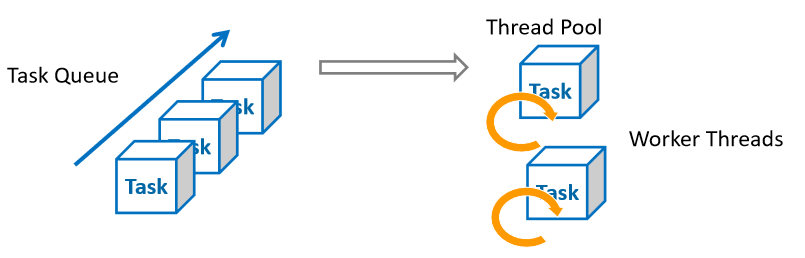
\includegraphics[width=\columnwidth]{Images/thread-pool}

\begin{lstlisting}
var pool = new ForkJoinPool();

// nicht blockierend
Future<Integer> future = pool.submit(() -> {
	// Task
	int value = ...;
	return value;
});
// oder
Integer future = pool.invoke(new MyRecursiveTask(value));

// blockierend
var res = future.get();
\end{lstlisting}
Beispiel um 3 Zahlen zu summieren welche nebeneinander in einem Array stehen.
\begin{lstlisting}
class ConvolutionTask extends RecursiveAction {
	private final int[] input;
	private final int[] output;
	private final int lower;
	private final int upper;
	private final static int THRESHOLD = 1000; // any value > 1
	public ConvolutionTask(int[] input, int[] output, int lower, int upper) {
		this.input = input;
		this.output = output;
		this.lower = lower;
		this.upper = upper;
	}
	@Override protected void compute() {
		if (upper - lower > THRESHOLD) {
			int middle = (lower + upper) / 2;
			invokeAll(
			new ConvolutionTask(input, output, lower, middle),
			new ConvolutionTask(input, output, middle, upper)
			);
		} else {
			for (int i = lower; i < upper; i++) {
				int left = i > 0 ? input[i - 1] : 0;
				int right = i < input.length - 1 ? input[i + 1] : 0;
				output[i] = left + input[i] + right;
			}
		}
	}
}
\end{lstlisting}

Ein \textbf{Daemon}-Thread hält das Programm nicht am leben. Daher müssen die Worker-Threads daemon sein, ansonsten würde das Programm nie beendet werden. Nachteil, Tasks sind nicht garantiert, dass sie abgearbeitet werden.


\subsection{Continuation}
\begin{lstlisting}
	CompletableFuture<Integer> future = CompletableFuture<Integer>.supplyAsync(()-> longOp());
	future.thenApply(result -> callWithReturn(result));
	future.thenAccept(result -> callNoReturn(result));
\end{lstlisting}


\subsection{.NET TPL}
In c\# gibt es eine Default Thread Pool welcher für 
\begin{enumerate}[nosep]
	\item Task: Explizite Tasks
	\item Data: Parallel Statements und Queries
	\item Asynchrone Programmierung
\end{enumerate}

\subsubsection{Parallel}
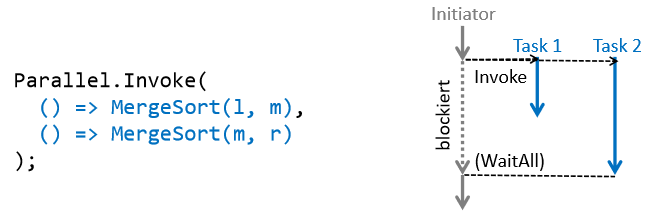
\includegraphics[width=\columnwidth]{Images/parallel_invoke}
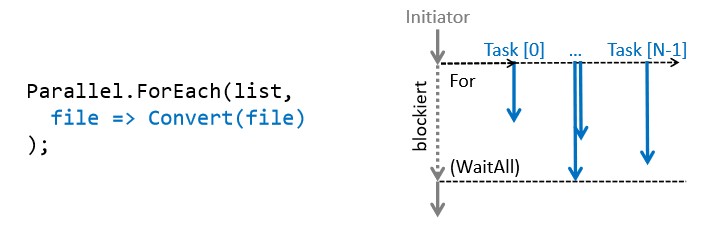
\includegraphics[width=\columnwidth]{Images/parallel_loop}

\section{Memory Model}
\subsection{Java}
In Java sind \textbf{atomare} Schreibe- und Leseinstruktionen nur für Primitive Datentypen bis 32-bit und Objekt-Referenzen garantiert. Long und Double Typen sind nur mit \underline{volatile} atomar.

Nur atomar bedeutet nicht, dass Thread B die Änderung auch mit bekommt. \textbf{Visibility} synchronisiert lese/schreibe Zugriff von volatile Variablen.

\begin{center}
	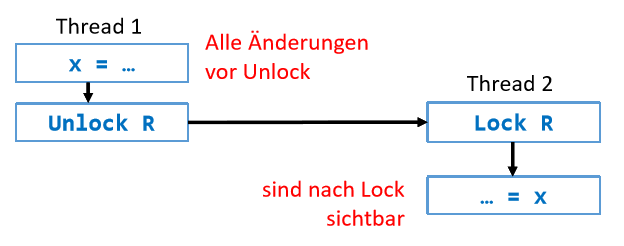
\includegraphics[width=0.6\columnwidth]{Images/visibility}
\end{center}

In Java sind zudem alle Synchronisations-Instruktionen total \textbf{ordered}, in c\# nicht! d.H in Java funktioniert folgendes Beispiel, in c\# nicht.
\begin{lstlisting}
volatile boolean a = false, b = false;

// Thread 1					// Thread 2
a = true;						b = true;
while(!b) {}				while(!a) {}
\end{lstlisting}

In c\# kann dies verhindert werden mit Thread.MemoryBarrier(), dies verhindert die Umordnung.
\begin{lstlisting}
volatile boolean a = false, b = false;

// Thread 1								// Thread 2
a = true;									b = true;
Thread.MemoryBarrier();		Thread.MemoryBarrier();
while(!b) {}							while(!a) {}
\end{lstlisting}


\subsection{Atomare Operationen}
In Java sind \textit{Atomic*} für *Integer, *Long, *Referenzen diversen Funktionen getAndSet(), addAndGet(), getAndAdd() oder compareAndSet(expect, update) etc atomar.


\section{GPU Programming}
CUDA für Nvidia Karten und OpenCL für HW-Unabhängig Programmierung von GPU.

\subsection{Performance}
Siehe auch Kapitel \ref{performance}.
\begin{center}
	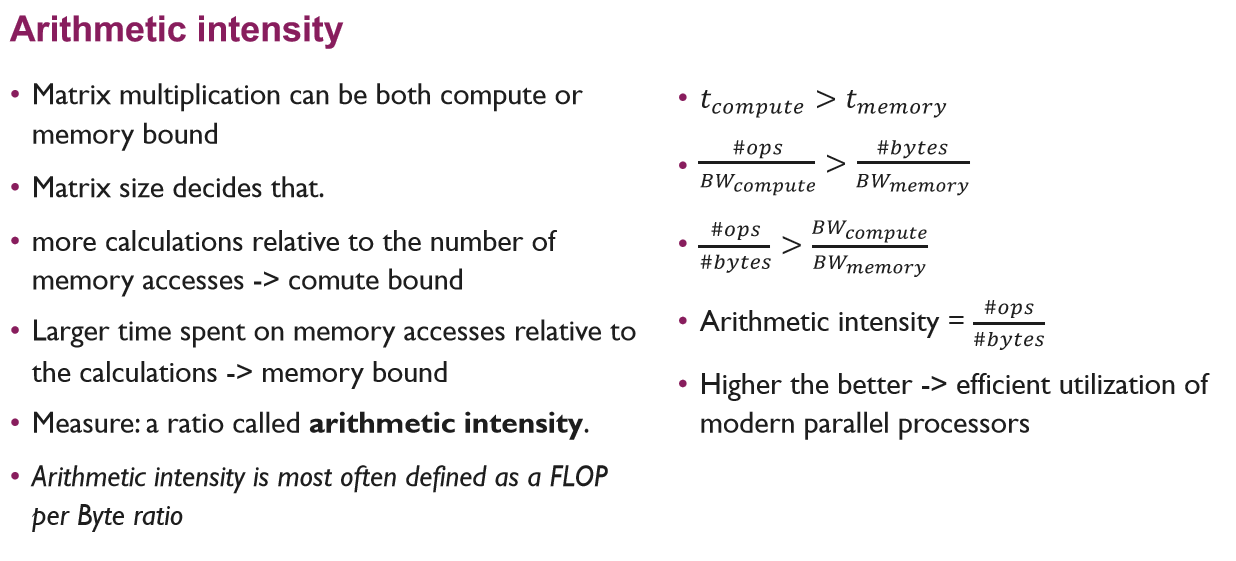
\includegraphics[width=\columnwidth]{Images/intensity}
\end{center}


\subsection{CUDA Execution Model}
CUDA ist in Blocks (auch Streaming Multiprocessor) aufgeteilt, welche wiederum aus \textit{Threads} (auch Streaming Processor) besteht. Jeder Thread hat eine eigene Id (x, y und z), um auf Daten zuzugreifen.

\begin{center}
	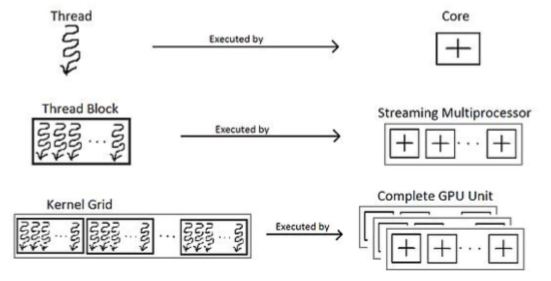
\includegraphics[width=0.9\columnwidth]{Images/gpu}
\end{center}

\begin{lstlisting}
// kernel definition for CUDA, executed on GPU
__global__ void parallelSum(int* array, int length) {
	int offset = blockIdx.x * blockDim.x;
	int stride = 1;
	while (stride < blockDim.x) {
		int first = offset + 2 * stride * threadIdx.x;
		int second = first + stride;
		if (second < length) {
			array[first] += array[second];
		}
		stride *= 2;
		__syncthreads();
	}
}

__global__ void matrixMultiply(float *A, float *B, float *C) {
	int col = blockIdx.x * blockDim.x + threadIdx.x;
	int row = blockIdx.y * blockDim.y + threadIdx.y;
	float sum = 0.0f;
	
	if (row < C_ROWS && col < C_COLS) {
		for (int k = 0; k < A_COLS; k++) {
			sum += A[row * A_COLS + k] * B[k * B_COLS + col];
		}
		
		C[row * C_COLS + col] = sum;
	}
}

// executet on CPU (Host)
int main() {
	// (1) alloc GPU memory
	cudaMalloc(..); 		
	// (2) transfer Data to GPU			
	cudaMemcpy(dst, src, size, dir); 
	// (3) kernel invocation	
	parallelSum<<<1, N>>>(A,B); 
	
    dim3 threadsPerBlock(tile_size, tile_size);
	dim3 blocksPerGrid((C_COLS + tile_size - 1) / tile_size, (C_ROWS + tile_size - 1) / tile_size);
	
	matrixMultiply<<<blocksPerGrid, threadsPerBlock>>>(d_a, d_b, d_c);
	
	// (4) transfer Data to CPU	
	cudaMemcpy(dst, src, size, dir); 
	// (5) free data	
	cudaFree(..);						
}
\end{lstlisting}

\subsection{Cuda Grid}
\textbf{threadIdx.x} greift auf Thread number im Block zu, \textbf{blockIdx.x} beinhaltet die Block Nummer und \textbf{blockDim.x} die Block grösse.
\begin{center}
\begin{lstlisting}
	int N = 32;
	dim3 grid = (8,4,2); // x, y, z => 64 blocks
	dim3 block = (N, 1, 1); // x, y, z => 32 threads per block
	VectorAddKernel<<<grid, block>>>(A,B,C);
	
	int threadsPerBlock = 256;
	int blocksPerGrid = (N + threadsPerBlock - 1) / threadsPerBlock;
	VectorAddKernel<<<blocksPerGrid, threadsPerBlock>>>(A,B,C);
\end{lstlisting}
	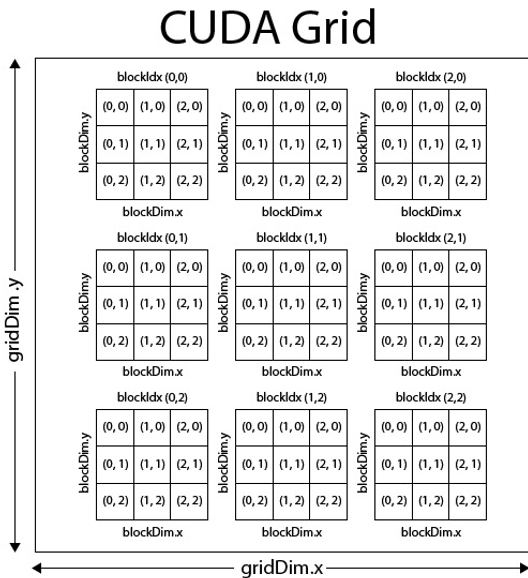
\includegraphics[width=0.6\columnwidth]{Images/grid}
\end{center}
Um auf die Daten in Array zuzugreifen kann pro Thread folgende Formel verwendet werden:
\[
index = blockIdx.x * blockDim.x + threadIdx.x
\]

\subsection{Performance}
\subsection{Divergence, Warp Exceution}
Alle Threads auf GPU sollten gleiche Instruktionen ausführen, sonst müssen diese aufeinander Warten und sind dadurch blockiert. Problem bei if/for/do/switch statements, weil diese Unterschiedliche Laufzeiten aufweisen können. Daher pro Warp gleiche Ausführung forcieren:
\begin{lstlisting}
if (threadIdx.x > 1) { } // BAD
if (threadIdx.x / 32 > 1) { } // GOOD
\end{lstlisting}

\subsection{Coalesing}
Pro Warp sollten auf gleiche Daten zugegriffen werden, um Performance zu erhöhen. Dies wird Coalescing genannt. Ein Zwischenfall ist Strided Coalescing.
\begin{center}
	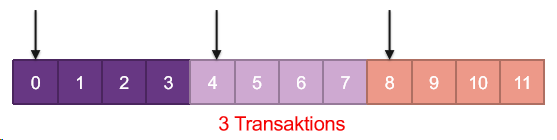
\includegraphics[width=0.8\columnwidth]{Sections/coalescing}
\end{center}

\section{MPI}

\subsection{Performance Analysis}
Für \textbf{strong} Speedup berechnungen folgende Formale kann verwendet werden:
$T = (1-p)T + Tp$ als Total Time, $p$ Fraction part $s = 1 -p$ serial Part mit $N$ Prozessoren.
\[
SpeedUp \leq \frac{T}{\frac{T\cdot p}{N} + (1-p)T} = \frac{1}{s + \frac{p}{N}}= \frac{1}{1-p + \frac{p}{N}}
\]
In dieser Formel sind keinen overhead mit einberechnet und ist daher nur eine theoretische maximaler Wert. Für den theoretischen \underline{Maximalen} Speedup $\lim\limits_{N\rightarrow\infty}$. Die \textbf{Effizienz} wird berechnet mit
\[
Efficiency = \frac{T}{N \cdot \underbrace{\left(\frac{T\cdot p}{N} + (1 - p)T\right)}_{T_N}}
\]

Für scaled speedup \textbf{weak} die Folgende Formel muss verwendet werden:
\[
SpeedUp = s + p\cdot N = s + (1-s)\cdot N
\]

\subsection{Flynn's Classical Taxonomy}
\noindent\begin{minipage}{\textwidth}
	\begin{minipage}{0.25\textwidth}
		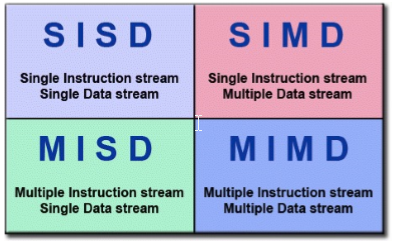
\includegraphics[width=\linewidth,keepaspectratio=true]{Images/flynn}
	\end{minipage}%%% to prevent a space
	\begin{minipage}{0.2\textwidth}
		SISD is used in a single core.\\
		SIMD für zB GPU\\
		MISD für failsafe Systeme\\
		MIMD für Clusters
	\end{minipage}
\end{minipage}

\subsection{Memory}
Es gibt grundsätzlich folgende Memory Typen:
\begin{enumerate}[nosep]
	\item Shared Memory
	\item Distributed Memory
	\item Hybrid Distributed-Shared Memory
\end{enumerate}

Oft ist der Memory-Throughput der Bottleneck. In modernen CPU, welche nach \textbf{Neumann Computer Architecture} gebaut sind, sind Instruktion und Data Memory am gleichen Bus angebunden. Im Gegensatz zu Embedded Geräten, welche nach \textbf{Harvard Architecture} zwei Buse existieren.
~\\~\\
Um diesen Problem entgegenzuwirken wird von UMA (Uniform memory access) zu NUMA (Non-Uniform memory access) gewechselt. Der Bus Interconnect verbindet muss sehr schnell sein (100GBit/s Ethernet), dies wird mit dem \textbf{MPI} umgesetzt. 
\begin{center}
	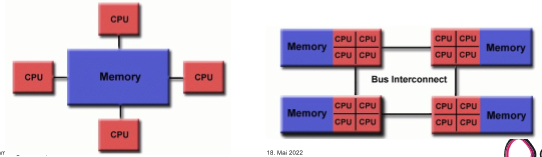
\includegraphics[width=0.6\columnwidth]{Images/uma}
\end{center}


\subsection{MPI API}
Die Anzahl Aktors sind fix beim Starten und können nicht zur Laufzeit geändert werden. Es gibt zudem auch kein Data Races, weil kein Shared Memory zwischen den Prozessen existiert.
\begin{tabular}{p{4cm}|p{4cm}}
	\textbf{MPI\_Barrier} & Warten, bis alle Prozesse Barrier erreicht haben \\
	\textbf{MPI\_Allreduce} & Aggregation von Teilresultaten zwischen Prozessoren, jeder erhält Gesamtresultat als Rückgabewert (inkl Broadcast) \\
	\textbf{MPI\_Reduce} & Aggregation von Teilresultaten zwischen Prozessoren, nur ein Prozess (rank) erhält Gesamtresultat \\
	\textbf{MPI\_Bcast} & Sendet Nachricht an mehrere Targets\\
	\textbf{MPI\_Send} & Sendet blockierend an Target \\
	\textbf{MPI\_Recv} & Empfängt blockierend von Sender \\
\end{tabular}

\subsubsection{Demo}
Der folgende Code muss mit \textit{mpicc -o app demo.c} kompiliert und mit \textit{mpiexec -n 32 app} ausgeführt werden. Dabei werden 32 von der gleichen Applikation gestartet verteilt auf den verfügbaren CPU.
\begin{lstlisting}
	#include <stdio.h> 
	#include "mpi.h" 
	
	int main(int argc, char* argv[]) {
		MPI_Init(&argc, &argv);
		
		int rank, size;
		MPI_Comm_rank(MPI_COMM_WORLD, &rank);
		MPI_Comm_size(MPI_COMM_WORLD, &size);
		char name[MPI_MAX_PROCESSOR_NAME];
		int len;
		MPI_Get_processor_name(name, &len);
		printf("Hello cluster from process %i on %s\n", rank, name);
		
		if (rank == 0) {
			int value = rand();
			for (int to = 1; to < size; to++) {
				MPI_Send(&value, 1, MPI_INT, to, 0 , MPI_COMM_WORLD);
			}
		} else {
			int value;
			MPI_Recv(&value, 1, MPI_INT, 0, 0, MPI_COMM_WORLD, MPI_STATUS_IGNORE);
			printf("%i received by %i", value, rank);
		}
		
		MPI_Finalize();
		
		return 0;
	}
\end{lstlisting}

\subsection{openMP}
OpenMP verwaltet Threads in einer MPI Umgebung, das zu einem Hybrid Model zwischen Threads und Nodes führt.

Das folgende Programm startet \textbf{OMP\_NUM\_THREADs} Threads pro Programm sobald pragma erreicht ist und führt den Folgenden Block parallel aus.
\begin{lstlisting}
#include <stdio.h>
#include <omp.h>
	
int main(int argc, char* argv[]) {
	const int np = omp_get_max_threads();
	printf("OpenMP with threads %d\n", np);
	
#pragma omp parallel
	{
		const int id = omp_get_thread_num();
		printf("Hello from thread %d\n", id);
	}

	return 0;
}
\end{lstlisting}

Um eine For-Schleife Parallel auszuführen kann ein \textit{for} nach dem pragma hinzugefügt werden. Variable A ist für jeden Thread private, B wird über alle Threads geshared (aber nicht synchronisiert)

\begin{lstlisting}
long hits = 0;
long i;
double x,y;
long count_hits(long trails) {
	#pragma omp parallel
	{
	#pragma omp parallel for reduction(+:hits) private (x,y)
		for (i = 0; i < trails; ++i) {
			x = random_double();
			y = random_double();
			if (x*x + y*y <= 1) hits++;
		}
	}
	return hits;
}	
\end{lstlisting}

\end{document}